\part{Telemetry System Design}

This year's telemetry system aims to address the shortcomings in last year's design. The main flaws that are being
addressed are:

\begin{itemize}
    \item Battery life status updates
    \item Power consumption
    \item System size for physical placement in the rocket
    \item Radio signal strength
    \item Enclosure integrity under shock load
    \item Lack of sensor fusion and equal data acquisition
    \item Use of memory for data logging while the rocket is idle
\end{itemize}

\section{Hardware Design}

\subsection{Power System}

\fxwarning{Add power system and arming design}

\subsection{Sensor Systems}

\fxwarning{Add sensor systems design}

\section{Software Design}

\subsection{Data Logging}

Data logging during flight will be done in a significantly more robust manner than previous years. This involves more
physically secure memory for logging, as well as power-failure guarantees. We will also be conserving space through
lift-off and landing detection.

\subsubsection{Data Integrity}

The physical memory being used for flight data logging is a standard microSD card. This memory was chosen because it is
cheap, ubiquitous, has an extremely large capacity and is easy to remove for data analysis on a computer immediately
after the rocket is recovered.

One of the challenges posed by an SD card is that it is designed to be removable in nature. SD card slots for quick
removal do not fare well in high vibration and high shock force environments like a rocket. They create a risk for the
SD card to fall out in flight, and also an opportunity for vibrations to temporarily break the electrical connection
between the card and the \gls{mcu}.

To address these risks, \gls{cuinspace} is securing the SD card in a cage-like slot, specifically manufactured to
survive shock loads of up to 50g and have electronic discontinuity for only up to 1 microsecond. An image of this
microSD slot can be seen in \Cref{fig:sd-card-cage}.

\begin{figure}[H]
    \centering
    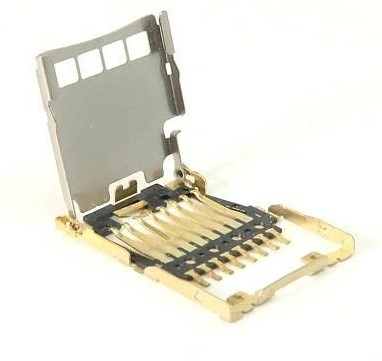
\includegraphics[width=2in]{./assets/images/sd-card-cage.jpg}
    \caption{Shock load resistant microSD card slot \cite{sd-card-cage}}
    \label{fig:sd-card-cage}
\end{figure}

In order to mitigate discontinuity risks on the software side, the microSD card will make use of the \textit{littlefs}
file system, which provides power-failure safety guarantees. Any brief discontinuity during a write to the SD card will
not corrupt any data, thus preserving the integrity of all logs. You can read more about \textit{littlefs} in
\Cref{apx:littlefs}.

In addition to the \textit{littlefs} file system on the microSD card, there will also be a FAT file system partition.
This partition allows for easy viewing of the telemetry data on a laptop immediately after recovery, as the FAT file
system is accessible through the file explorer on both Windows and Linux computers. Logged flight data is copied from
the \textit{littlefs} partition to the FAT partition upon landing, when there is very little risk of vibrations
corrupting the transfer. The FAT partition will be the first partition on the microSD's partition table so that it is
detected properly on Windows machines.

\subsubsection{Logging Space Conservation}

In order to preserve logging space and avoid filling up memory with telemetry data being collected while the rocket is
idle on the launch rail, we will be using lift-off and landing detection to trigger logging operations. The state
machine used to govern this portion of the system can be seen in \Cref{fig:logging-fsm}.

\begin{figure}[H]
    \centering
    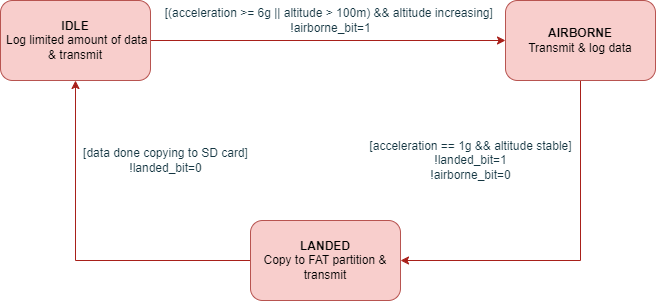
\includegraphics[width=4in]{./assets/diagrams/Flight State FSM.png}
    \caption{Logging control finite state machine}
    \label{fig:logging-fsm}
\end{figure}

Last year, much of the logged telemetry data was captured while the rocket was idle on the launch rail. This is the
\textit{IDLE} state in \Cref{fig:logging-fsm}. In this state we continue to transmit telemetry because it's necessary
to confirm the system's operation and a stable radio signal, but we do not log continuously. Instead, logs are recorded
for only the past 30 seconds at any given time. This gives the system breathing room for latency when detecting
lift-off, without losing any critical data about the start of the launch.

Lift-off is detected using the accelerometer data in conjunction with the barometric pressure sensor. The accelerometer
data can detect the high g-force experienced at launch (previous launches have seen up to 24g) and the barometric
pressure sensor can detect a climbing altitude. In the first few seconds of lift-off, the system will be able to detect
the high g-force and increasing acceleration, at which point it will move to the \textit{AIRBORNE} state. This state is
recorded by setting the "airborne bit" to 1 in the on-board \gls{eeprom}. Doing so means that if the system experience
power-failure in the air, when it reboots it will successfully boot into the \textit{AIRBORNE} state again.

In the \textit{AIRBORNE} state, the flight computer will continuously log to the \textit{littlefs} partition on the SD
card. This will capture flight data at a much higher frequency than is possible to transmit over radio.

Eventually, once the rocket has deployed its chutes at apogee and descended to the ground, the system will detect
landing. The criteria for landing detection is an accelerometer reading of maximum 1g (with slight tolerance for noise)
in any axes combined with a stable altitude which is at ground level. This should prevent landing detection from
triggering while the rocket is at apogee or descending slowly, at which point its altitude will still be quite high and
it should be descending at a larger acceleration than 1g. These thresholds will be configurable and will be set prior
to flight based on simulations on descent speed by the recovery team.

Once the landing is detected, the system will enter the \textit{LANDED} state. In this state the "airborne bit" will be
set to 0 and the "landed bit" will be set to 1. The system will begin copying all logged flight data from the
\textit{littlefs} partition to the FAT filesystem partition on the SD card. During this time it continues to transmit
telemetry over radio.

Once all the data is copied over, the "landed bit" will be set to 0, and the system will re-enter the \textit{IDLE}
state. At this point, the system still continues transmitting GPS coordinates for recovery, and all flight logs are
safe on the SD card for post-flight extraction. Logs on the \textit{littlefs} partition are only over-written when the
system re-enters the \textit{AIRBORNE} state, which is not possible to trigger from the ground.

\section{Radio Frequency Design}

\section{Enclosure Design}

%This might be in aerostructures PDR, not certain.
